%% ----------------------------------------------------------------------------
%%  §10.1  Il resto di Peano. Nuovi sviluppi
%% ----------------------------------------------------------------------------
\section{Il resto di Peano}
\label{sec:taylor-peano}

\subsection{Polinomi e loro sviluppi}

Consideriamo un polinomio di grado $n$ a coefficienti reali,
$p(x)=a_{0}+a_{1}x+a_{2}x^{2}+\dots+a_{n}x^{n}$. La funzione $p$ è derivabile infinite volte in
$\R$, le sue derivate di ordine maggiore di $n$ sono tutte nulle, e, come nella
dimostrazione del \cref{lem:derivate-taylor}, $p^{(k)}(0)=k!\,a_{k}$ per ogni $k\le n$.
Ricavando i coefficienti, il polinomio si scrive
\begin{equation}\label{eq:polinomio-mac-laurin}
  p(x)=p(0)+\frac{p'(0)}{1!}\,x+\frac{p''(0)}{2!}\,x^{2}+\dots+\frac{p^{(n)}(0)}{n!}\,x^{n} :
\end{equation}
un polinomio di grado $n$ è noto una volta noti il suo valore e quelli delle sue prime
$n$ derivate nello zero. Lo stesso vale per un qualsiasi punto $x_{0}$.

\begin{proposizione}[Un polinomio coincide con il proprio sviluppo]
\label{prop:polinomio-sviluppo}
Sia $p$ un polinomio di grado $\le n$ e sia $x_{0}\in\R$. Allora
\begin{equation}\label{eq:polinomio-sviluppo}
  p(x)=\sum_{k=0}^{n}\frac{p^{(k)}(x_{0})}{k!}\,(x-x_{0})^{k} \qquad\perogni x\in\R .
\end{equation}
In particolare, un polinomio di grado $\le n$ è univocamente determinato dai valori che
esso e le sue prime $n$ derivate assumono in $x_{0}$.
\end{proposizione}

\begin{schema}
\Ipotesi{$p$ polinomio di grado $\le n$; \ $x_{0}\in\R$.}
\Tesi{$p(x)=\sum_{k=0}^{n}\frac{p^{(k)}(x_{0})}{k!}(x-x_{0})^{k}$ per ogni $x$: il resto della formula di
Taylor di ordine $n$ è identicamente nullo.}
\end{schema}

\begin{strategia}
Si cambia variabile ponendo $h=x-x_{0}$: il polinomio $q(h)=p(x_{0}+h)$, sviluppati i
binomi, è un polinomio di grado $\le n$ in $h$, e per esso vale la
\eqref{eq:polinomio-mac-laurin}. Resta da osservare che le derivate di $q$ in $0$ sono quelle
di $p$ in $x_{0}$.
\end{strategia}

\begin{dimostrazione}
Sia $q(h)=p(x_{0}+h)$. Sviluppando ciascuna potenza $(x_{0}+h)^{j}$ con la formula del binomio
(\cref{teo:binomio}) e raccogliendo, $q$ è un polinomio di grado $\le n$ nella variabile
$h$, diciamo $q(h)=\sum_{k=0}^{n}c_{k}h^{k}$, e quindi $c_{k}=\frac{q^{(k)}(0)}{k!}$. Per la regola di
derivazione delle funzioni composte (con la funzione interna $h\mapsto x_{0}+h$, di derivata
$1$), $q^{(k)}(h)=p^{(k)}(x_{0}+h)$, e in particolare $q^{(k)}(0)=p^{(k)}(x_{0})$. Dunque
$p(x)=q(x-x_{0})=\sum_{k=0}^{n}\frac{p^{(k)}(x_{0})}{k!}(x-x_{0})^{k}$. L'ultima affermazione segue
perché il secondo membro dipende soltanto dai numeri $p^{(k)}(x_{0})$.
\end{dimostrazione}

Ad esempio, il polinomio $p(x)=x^{3}$ ha in $x_{0}=1$ le derivate $p(1)=1$, $p'(1)=3$,
$p''(1)=6$, $p'''(1)=6$, e quindi $x^{3}=1+3(x-1)+3(x-1)^{2}+(x-1)^{3}$, come si verifica
anche con la formula del binomio applicata a $\bigl(1+(x-1)\bigr)^{3}$.

\begin{notastorica}[Taylor, Mac Laurin e le differenze finite]
Taylor arrivò al suo sviluppo partendo da un analogo «discreto» della
\cref{prop:polinomio-sviluppo}. Fissato un passo $h$, le \emph{differenze in avanti}
$\Delta f(x_{0})=f(x_{0}+h)-f(x_{0})$, $\Delta^{2}f(x_{0})=\Delta f(x_{0}+h)-\Delta f(x_{0})$, \dots\
ricostruiscono i valori di $f$ nei punti $x_{0}+mh$ mediante la formula di interpolazione
di Newton (\emph{Principia}, 1687, già in una lettera di James Gregory del 1670):
\[
\begin{aligned}
  f(x_{0}+mh)&=\sum_{k=0}^{m}\binom mk\Delta^{k}f(x_{0})\\
  &=\sum_{k=0}^{m}\frac{v(v-h)\cdots\bigl(v-(k-1)h\bigr)}{k!}\cdot\frac{\Delta^{k}f(x_{0})}{h^{k}} ,
\end{aligned}
\]
dove $v=mh$. Taylor, che annunciò il teorema in una lettera del 26 luglio 1712 a John
Machin (lo stesso della formula \eqref{eq:machin}), fissò $v=x-x_{0}$ e lasciò «svanire»
gli incrementi: per $h\to0$ il primo fattore diventa $\frac{(x-x_{0})^{k}}{k!}$ e il secondo la
flussione, cioè la derivata $f^{(k)}(x_{0})$. Ecco l'origine dei coefficienti
$\frac{f^{(k)}(x_{0})}{k!}$; ma il passaggio al limite non era giustificato, perché il numero
dei termini cresce con $m$. Mac Laurin, nel \emph{Treatise of Fluxions} (1742), scritto per
rispondere alle critiche di Berkeley (\S\ref{sec:def-limite}), seguì un'altra strada:
supposto $f(x)=A+Bx+Cx^{2}+\cdots$, derivò ripetutamente e pose $x=0$, esattamente come
per la \eqref{eq:polinomio-mac-laurin}, riconoscendo che la formula era un caso
particolare di quella di Taylor; essa compariva già nel \emph{Methodus differentialis}
(1730) di James Stirling. Né Taylor né Mac Laurin si chiesero quanto valesse l'errore
commesso arrestando la somma: è la domanda a cui risponde questo capitolo.
\end{notastorica}

Sia ora $f$ una funzione derivabile $n$ volte in un punto $x_{0}$ (nel senso della
\cref{not:derivabile-n-volte}). Per la \cref{prop:polinomio-sviluppo}, il polinomio di
grado $\le n$ che ha nel punto $x_{0}$ lo stesso valore e le stesse prime $n$ derivate di
$f$ esiste, è unico, ed è il polinomio di Taylor $T_{n}$ della
\eqref{eq:polinomio-taylor}. La funzione $R_{n}(x)=f(x)-T_{n}(x)$, il \emph{resto}, rappresenta
l'errore che si commette sostituendo a $f(x)$ il suo polinomio di Taylor, e il
\cref{teo:taylor} afferma che
\begin{equation}\label{eq:peano-richiamo}
  f(x)=\sum_{k=0}^{n}\frac{f^{(k)}(x_{0})}{k!}(x-x_{0})^{k}+o\bigl((x-x_{0})^{n}\bigr)
  \qquad (x\to x_{0}) .
\end{equation}
Ricordiamo che la dimostrazione data nel \cref{sec:taylor} richiede soltanto l'esistenza
di $f^{(n)}(x_{0})$, e non la continuità di $f^{(n)}$ in $x_{0}$. Ad esempio, la funzione
$f(x)=x^{4}\sen\frac1x$, prolungata con $f(0)=0$, ha $f'(0)=f''(0)=0$, ma $f''$ non è continua
in $0$ (per $x\neq0$ contiene il termine $-\sen\frac1x$, che oscilla); la formula di Taylor di
ordine $2$ dice che $f(x)=o(x^{2})$, come è evidente da $\abs{f(x)}\le x^{4}$.

\subsection{Nuovi sviluppi senza calcolare derivate}

Calcolare le derivate successive di una funzione composta è in genere laborioso. Per la
\cref{prop:unicita-taylor}, però, \emph{qualunque} procedimento produca un polinomio di grado
$\le n$ che approssima $f$ con un errore $o\bigl((x-x_{0})^{n}\bigr)$ fornisce il polinomio di
Taylor. I due procedimenti più utili sono la sostituzione e l'integrazione.

\begin{lemma}[Sostituzione negli o piccoli]\label{lem:sostituzione-o}
Sia $g(t)=o(t^{m})$ per $t\to0$, e sia $\varphi$ una funzione con $\varphi(x)\to0$ per $x\to x_{0}$ e
$\varphi(x)\neq0$ per $x\neq x_{0}$. Allora $g\bigl(\varphi(x)\bigr)=o\bigl(\varphi(x)^{m}\bigr)$ per $x\to x_{0}$.
\end{lemma}

\begin{schema}
\Ipotesi{$\frac{g(t)}{t^{m}}\to0$ per $t\to0$; \ $\varphi(x)\to0$, $\varphi(x)\neq0$ per $x\neq x_{0}$.}
\Tesi{$\frac{g(\varphi(x))}{\varphi(x)^{m}}\to0$ per $x\to x_{0}$.}
\end{schema}

\begin{strategia}
Il rapporto $\frac{g(\varphi(x))}{\varphi(x)^{m}}$ è la funzione $\frac{g(t)}{t^{m}}$ calcolata in $t=\varphi(x)$: è il
teorema sul limite delle funzioni composte.
\end{strategia}

\begin{dimostrazione}
Posto $h(t)=\frac{g(t)}{t^{m}}$ per $t\neq0$, si ha $h(t)\to0$ per $t\to0$, e
$\frac{g(\varphi(x))}{\varphi(x)^{m}}=h(\varphi(x))$, con $\varphi(x)\to0$ e $\varphi(x)\neq0$ per $x\neq x_{0}$. Per il
teorema sul limite delle funzioni composte (\cref{teo:limite-composta}), $h(\varphi(x))\to0$.
\end{dimostrazione}

Ad esempio, da $\sen t=t-\frac{t^{3}}6+o(t^{4})$ \eqref{eq:taylor-sen}, con $t=x^{2}$ e $t=x^{3}$ si
ottiene
\begin{equation}\label{eq:sen-x2-x3}
  \sen x^{2}=x^{2}-\frac{x^{6}}6+o(x^{8}), \qquad \sen x^{3}=x^{3}-\frac{x^{9}}6+o(x^{12}) ,
\end{equation}
e in particolare $\sen x^{2}=x^{2}+o(x^{4})$ e $\sen x^{3}=x^{3}+o(x^{6})$: vicino a $0$ le funzioni
$\sen x^{2}$ e $\sen x^{3}$ hanno un «comportamento» simile a quello di $x^{2}$ e di $x^{3}$
(\cref{fig:taylor-composte}). Allo stesso modo, con $e^{x}-1=x+\frac{x^{2}}2+\frac{x^{3}}6+o(x^{3})$ e
$\sen u=u-\frac{u^{3}}6+o(u^{3})$, si trova
\[
  1+\sen\bigl(e^{x}-1\bigr)=1+x+\frac{x^{2}}2+o(x^{3}) ,
\]
perché il termine $\frac{x^{3}}6$ dello sviluppo di $e^{x}-1$ si elide con il $-\frac{u^{3}}6=-\frac{x^{3}}6+o(x^{3})$
del seno (le regole di calcolo degli o piccoli che stiamo usando saranno giustificate nel
\cref{sec:o-piccoli}): la funzione $1+\sen(e^{x}-1)$ ha in $0$ lo stesso polinomio di Taylor di ordine $2$
di $e^{x}$, e i due grafici sono simili vicino all'origine, mentre lontano da essa si
comportano in modo completamente diverso.

\begin{figure}[htb]
\centering
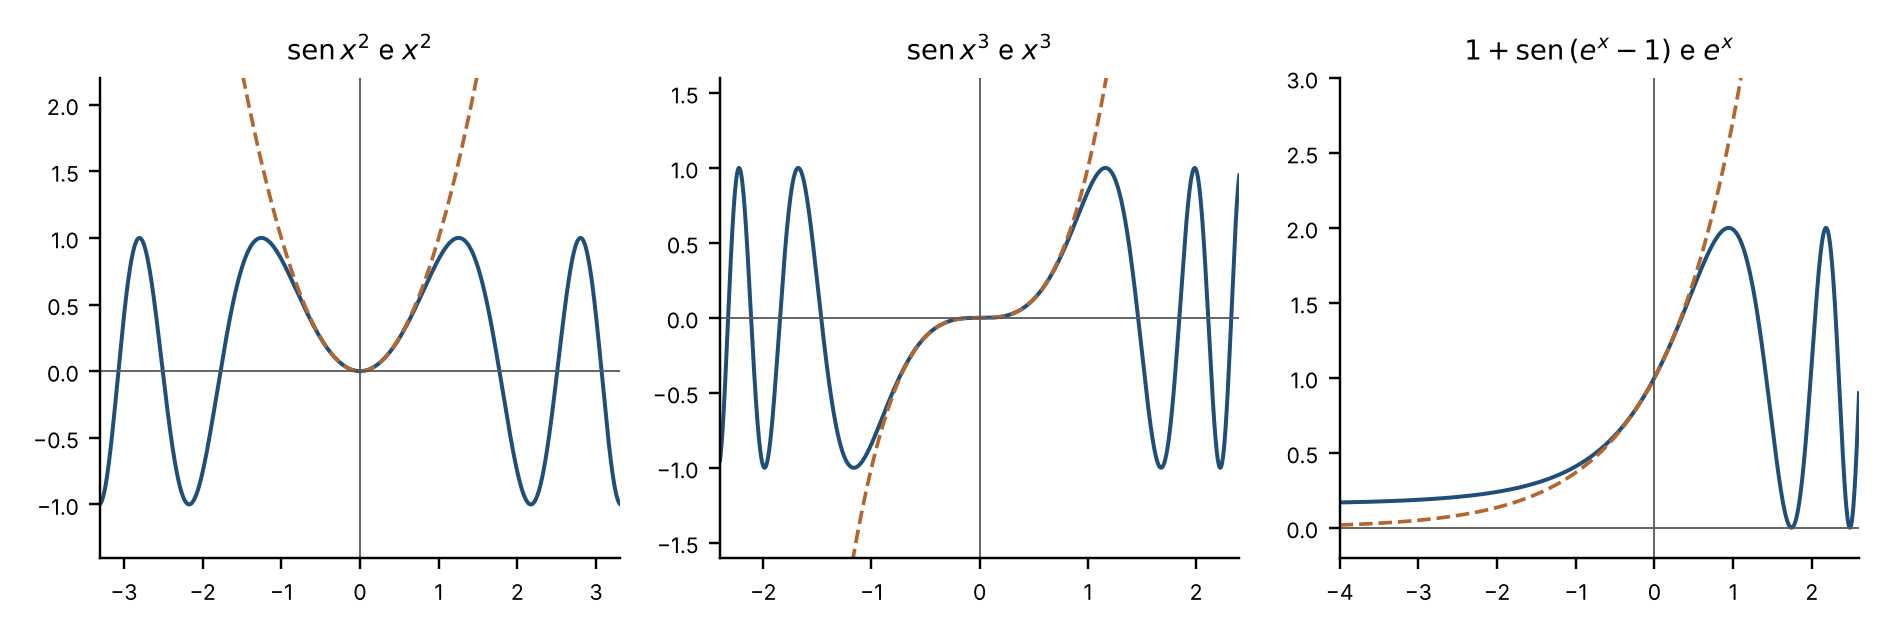
\includegraphics[width=\textwidth]{figure/taylor_composte.png}
\caption{Le funzioni $\sen x^{2}$, $\sen x^{3}$ e $1+\sen(e^{x}-1)$ (in blu) e le loro approssimazioni
vicino all'origine $x^{2}$, $x^{3}$, $e^{x}$ (tratteggio rame). Lontano dall'origine la
somiglianza scompare: $\sen x^{2}$ e $\sen x^{3}$ oscillano sempre più rapidamente, e
$1+\sen(e^{x}-1)$ oscilla per $x\to+\infty$ mentre tende a $1+\sen(-1)>0$ per $x\to-\infty$
(\texttt{python/fig\_taylor\_composte.py}).}
\label{fig:taylor-composte}
\end{figure}

Il secondo procedimento consiste nell'integrare uno sviluppo noto.

\begin{lemma}[Integrazione degli o piccoli]\label{lem:integrazione-o}
Sia $m\ge0$ un intero, e sia $g$ continua in un intorno $I$ di $0$, con $g(t)=o(t^{m})$ per
$t\to0$. Allora
\begin{equation}\label{eq:integrazione-o}
  \int_{0}^{x}g(t)\,dt=o(x^{m+1}) \qquad (x\to0) .
\end{equation}
\end{lemma}

\begin{schema}
\Ipotesi{$m\ge0$ intero; \ $g$ continua in $I\ni0$; \ $\frac{g(t)}{t^{m}}\to0$ per $t\to0$.}
\Tesi{$\frac1{x^{m+1}}\int_{0}^{x}g(t)\,dt\to0$ per $x\to0$.}
\end{schema}

\begin{strategia}
Vicino a $0$ si ha $\abs{g(t)}\le\epsilon\abs t^{m}$; integrando la disuguaglianza tra $0$ e $x$ si
ottiene una stima con $\frac{\epsilon\abs x^{m+1}}{m+1}$.
\end{strategia}

\begin{dimostrazione}
Sia $\epsilon>0$. Per l'ipotesi esiste $\delta>0$, che possiamo scegliere in modo che
$(-\delta,\delta)\subseteq I$, tale che $\abs{g(t)}\le\epsilon\abs t^{m}$ per $\abs t<\delta$
(anche per $t=0$, perché $g(0)=\lim_{t\to0}g(t)=0$ per la continuità). Per $0<\abs x<\delta$, per il
\cref{teo:valore-assoluto} e il confronto, applicati nell'intervallo di estremi $0$ e $x$,
\[
  \Bigl|\int_{0}^{x}g(t)\,dt\Bigr|\le\Bigl|\int_{0}^{x}\epsilon\abs t^{m}\,dt\Bigr|=\frac{\epsilon\abs x^{m+1}}{m+1}\le\epsilon\abs x^{m+1} ,
\]
cioè $\Bigl|\frac1{x^{m+1}}\int_{0}^{x}g\Bigr|\le\epsilon$, che è la tesi.
\end{dimostrazione}

Ne segue che uno sviluppo della derivata si può integrare «termine a termine»: se $f'$ è
continua vicino a $0$ e $f'(x)=\sum_{k=0}^{n}a_{k}x^{k}+o(x^{n})$, allora, per la formula
fondamentale e il lemma,
\begin{equation}\label{eq:integrazione-termine}
  f(x)=f(0)+\int_{0}^{x}f'(t)\,dt=f(0)+\sum_{k=0}^{n}\frac{a_{k}}{k+1}\,x^{k+1}+o(x^{n+1}) .
\end{equation}
Il procedimento inverso, cioè derivare uno sviluppo termine a termine, non è lecito in
generale: $x^{3}\sen\frac1x=o(x^{2})$, ma la sua derivata $3x^{2}\sen\frac1x-x\cos\frac1x$ non è $o(x)$.

\subsection{Lo sviluppo dell'arcotangente}

Applichiamo l'idea dell'integrazione all'arcotangente, le cui derivate successive sono
sempre più complicate. Il punto di partenza è che la sua derivata $\frac1{1+t^{2}}$ è la somma
di una progressione geometrica di ragione $-t^{2}$, a meno di un resto esplicito; in questo
modo otteniamo non soltanto lo sviluppo, ma anche una stima del resto valida per
\emph{ogni} $x$.

\begin{proposizione}[Sviluppo dell'arcotangente]\label{prop:sviluppo-arctg}
Per ogni $n\in\N\cup\set0$ e ogni $x\in\R$,
\begin{equation}\label{eq:sviluppo-arctg}
\begin{gathered}
  \operatorname{arctg}x=x-\frac{x^{3}}3+\frac{x^{5}}5-\dots+(-1)^{n}\frac{x^{2n+1}}{2n+1}+R(x),\\
  R(x)=(-1)^{n+1}\int_{0}^{x}\frac{t^{2n+2}}{1+t^{2}}\,dt, \qquad
  \abs{R(x)}\le\frac{\abs x^{2n+3}}{2n+3} .
\end{gathered}
\end{equation}
In particolare $R(x)=o(x^{2n+2})$ per $x\to0$, e il polinomio a secondo membro è il polinomio
di Taylor di ordine $2n+2$ dell'arcotangente in $0$.
\end{proposizione}

\begin{schema}
\Ipotesi{$n\ge0$ intero; \ $x\in\R$.}
\Tesi{la \eqref{eq:sviluppo-arctg}, con il resto in forma integrale e
$\abs{R(x)}\le\frac{\abs x^{2n+3}}{2n+3}$; \ $R(x)=o(x^{2n+2})$.}
\end{schema}

\begin{strategia}
La somma della progressione geometrica $1-t^{2}+t^{4}-\dots+(-1)^{n}t^{2n}$ è
$\frac{1-(-t^{2})^{n+1}}{1+t^{2}}$: dunque $\frac1{1+t^{2}}$ è uguale a questa somma più il resto esplicito
$\frac{(-1)^{n+1}t^{2n+2}}{1+t^{2}}$. Integrando tra $0$ e $x$, la somma dà il polinomio e il resto si
stima con $t^{2n+2}$, perché $1+t^{2}\ge1$. L'unicità del polinomio di Taylor fa il resto.
\end{strategia}

\begin{dimostrazione}
Per la formula della somma della progressione geometrica (\cref{prop:geometrica}) con
ragione $-t^{2}\neq1$,
\[
  \sum_{k=0}^{n}(-t^{2})^{k}=\frac{1-(-t^{2})^{n+1}}{1+t^{2}} ,
\]
cioè
\[
  \frac1{1+t^{2}}=\sum_{k=0}^{n}(-1)^{k}t^{2k}+(-1)^{n+1}\frac{t^{2n+2}}{1+t^{2}} .
\]
Integriamo tra $0$ e $x$: per la formula fondamentale, poiché $D\operatorname{arctg}t=\frac1{1+t^{2}}$
\eqref{eq:derivata-arctg} e $\operatorname{arctg}0=0$,
\[
  \operatorname{arctg}x=\sum_{k=0}^{n}(-1)^{k}\frac{x^{2k+1}}{2k+1}+R(x), \qquad
  R(x)=(-1)^{n+1}\int_{0}^{x}\frac{t^{2n+2}}{1+t^{2}}\,dt .
\]
Poiché $0\le\frac{t^{2n+2}}{1+t^{2}}\le t^{2n+2}$, per il confronto
$\abs{R(x)}\le\bigl|\int_{0}^{x}t^{2n+2}\,dt\bigr|=\frac{\abs x^{2n+3}}{2n+3}$. Ne segue
$\bigl|\frac{R(x)}{x^{2n+2}}\bigr|\le\frac{\abs x}{2n+3}\to0$, cioè $R(x)=o(x^{2n+2})$; per la
\cref{prop:unicita-taylor} il polinomio trovato è il polinomio di Taylor di ordine $2n+2$.
\end{dimostrazione}

Lo stesso ragionamento, con $\frac1{1+t}=\sum_{k=0}^{n-1}(-t)^{k}+\frac{(-t)^{n}}{1+t}$ ($n\ge1$), ritrova lo
sviluppo \eqref{eq:taylor-log} del logaritmo, con il resto
$R(x)=(-1)^{n}\int_{0}^{x}\frac{t^{n}}{1+t}\,dt$ e la stima $\abs{R(x)}\le\frac{x^{n+1}}{n+1}$ per ogni $x\ge0$ (per
$-1<x<0$ si trova invece $\abs{R(x)}\le\frac{\abs x^{n+1}}{(n+1)(1+x)}$).

La stima della \cref{prop:sviluppo-arctg} dice di più del resto di Peano. Se $\abs x\le1$,
il resto tende a zero per $n\to+\infty$: il valore di $\operatorname{arctg}x$ è il limite dei
polinomi. Per $x=1$ si ottiene la \emph{serie di Leibniz}
\begin{equation}\label{eq:serie-leibniz}
  \frac\pi4=\operatorname{arctg}1=1-\frac13+\frac15-\frac17+\cdots ,
\end{equation}
nel senso che le somme parziali differiscono da $\frac\pi4$ al più di $\frac1{2n+3}$. La
convergenza è però lentissima: per garantire un errore su $\pi$ inferiore a $10^{-6}$ la
stima richiede circa due milioni di termini. Molto più efficiente è la
\emph{formula di Machin}
\begin{equation}\label{eq:machin}
  \frac\pi4=4\operatorname{arctg}\frac15-\operatorname{arctg}\frac1{239}
\end{equation}
(che si verifica con la formula di addizione della tangente, \cref{es:machin}): con
$x=\frac15$ il resto è al più $\frac{5^{-(2n+3)}}{2n+3}$, e ogni termine aggiunge circa una cifra e
mezza. Se invece $\abs x>1$ la stima non serve, e infatti i polinomi di Taylor
dell'arcotangente si allontanano dalla funzione al crescere del grado
(\cref{fig:taylor-arctg}): a differenza di quanto accade per il seno
(\cref{fig:taylor-seno}), un'ottima approssimazione vicino a $0$ non garantisce nulla
lontano da $0$, anche per una funzione derivabile infinite volte su tutto $\R$. La ragione profonda di questo
comportamento è nascosta nel campo complesso: la funzione $\frac1{1+t^{2}}$, derivata
dell'arcotangente, non è definita nei numeri complessi $t=\pm i$, che distano $1$
dall'origine. La chiarisce la teoria delle serie di potenze, che si studia nei corsi
successivi e a cui accenneremo alla fine del \cref{cap:serie}.

\begin{figure}[htb]
\centering
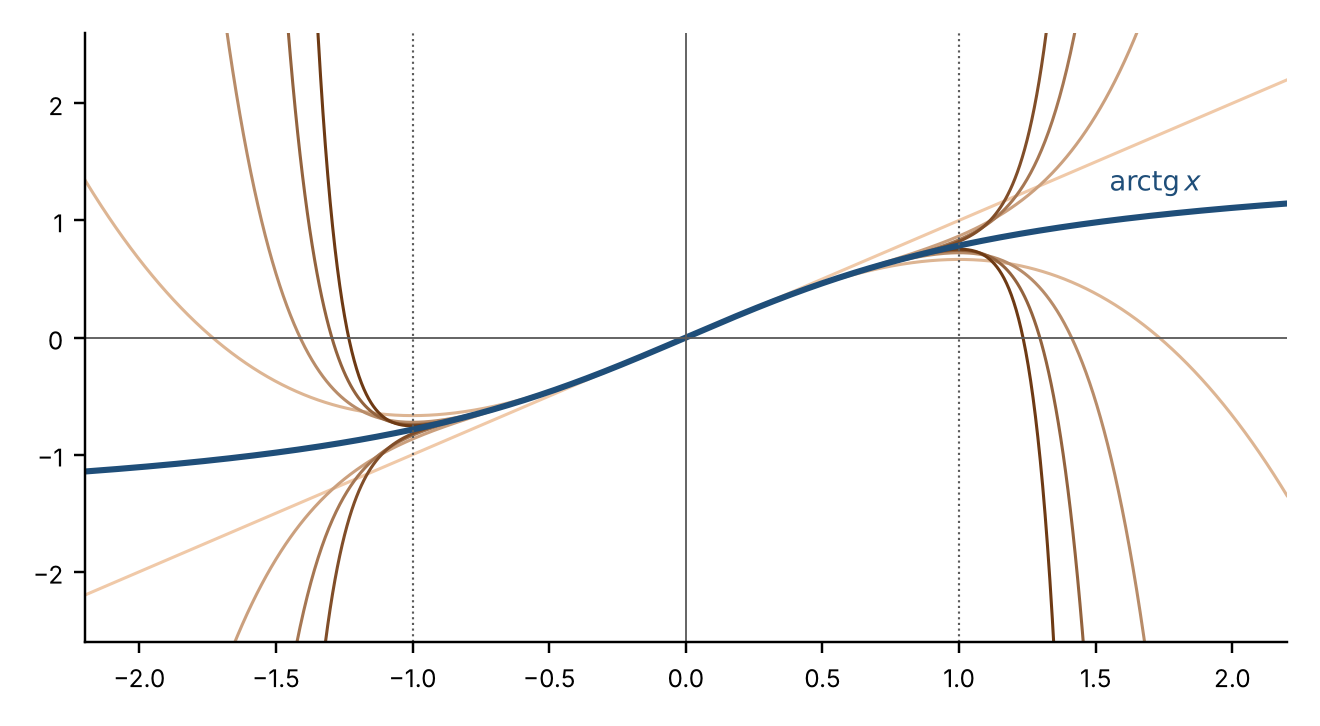
\includegraphics[width=\textwidth]{figure/taylor_arctg.png}
\caption{L'arcotangente (blu) e i suoi polinomi di Taylor in $0$ di grado $1,3,5,\dots,15$
(rame, più scuri al crescere del grado). In $[-1,1]$ i polinomi si avvicinano alla
funzione; per $\abs x>1$ se ne allontanano sempre di più
(\texttt{python/fig\_taylor\_arctg.py}).}
\label{fig:taylor-arctg}
\end{figure}

\begin{python}[Le cifre di $\pi$: serie di Leibniz e formula di Machin]
from fractions import Fraction as F
import math

def arctg(x, n):
    """T(x) = x - x^3/3 + ... + (-1)^n x^(2n+1)/(2n+1)."""
    return sum((-1)**k * x**(2*k + 1) / (2*k + 1)
               for k in range(n + 1))

for n in (10, 100, 1000):
    print(f"Leibniz, n = {n:4d}:  4*T = {4 * arctg(1.0, n):.10f}")
for n in (2, 4, 6, 8):
    p = 4 * (4 * arctg(F(1, 5), n) - arctg(F(1, 239), n))
    print(f"Machin,  n = {n}:     4*T = {float(p):.15f}")
print(f"                  pi    = {math.pi:.15f}")
\end{python}
\begin{risultato}
Leibniz, n =   10:  4*T = 3.2323158094
Leibniz, n =  100:  4*T = 3.1514934011
Leibniz, n = 1000:  4*T = 3.1425916543
Machin,  n = 2:     4*T = 3.141621029325035
Machin,  n = 4:     4*T = 3.141592682404399
Machin,  n = 6:     4*T = 3.141592653623555
Machin,  n = 8:     4*T = 3.141592653589836
                  pi    = 3.141592653589793
\end{risultato}

\begin{idea}[La distanza dell'orizzonte]
Da un velivolo che vola alla quota $h$ sopra una Terra sferica di raggio
$R\approx6371$~km, la visuale verso l'orizzonte è tangente alla superficie
(\cref{fig:orizzonte}). Se $\vartheta$ è l'angolo al centro della Terra tra la verticale del
velivolo e il punto di tangenza, il triangolo rettangolo formato dal centro, dal velivolo
e dal punto di tangenza dà $\cos\vartheta=\frac R{R+h}$, cioè $1-\cos\vartheta=\frac h{R+h}$, e la
distanza dell'orizzonte misurata sulla superficie è $d=R\vartheta$. Per la
\eqref{eq:taylor-cos}, $1-\cos\vartheta=\frac{\vartheta^{2}}2\,(1+o(1))$ per $\vartheta\to0$; poiché $h$ è piccolo
rispetto a $R$, anche $\vartheta$ è piccolo, e
\begin{equation}\label{eq:orizzonte}
  \vartheta\approx\sqrt{\frac{2h}{R}}, \qquad d\approx\sqrt{2Rh} .
\end{equation}
A $10\,000$~m di quota l'orizzonte dista circa $\sqrt{2\cdot6371\cdot10}\approx357$~km. La stessa
formula dà la portata «ottica» di un radar o di un collegamento radio in visibilità; in
radiotecnica, per tener conto della rifrazione atmosferica, si usa un raggio terrestre
equivalente pari ai $\frac43$ di quello reale. Il programma confronta la formula
approssimata con quella esatta $d=R\arccos\frac R{R+h}$. Si vedrà che l'approssimazione
sovrastima leggermente la distanza; l'\cref{es:orizzonte-secondo-ordine} ne spiega il
motivo e ne calcola l'errore.
\end{idea}

\begin{figure}[htb]
\centering
\begin{tikzpicture}[scale=1.0]
  \fill[blu!8] (0,0) circle (2.2);
  \draw[blu, thick] (0,0) circle (2.2);
  \coordinate (O) at (0,0);
  \coordinate (A) at (0,3.3);
  \coordinate (T) at ({2.2*sin(48.19)},{2.2*cos(48.19)});
  \draw[grigio] (O) -- (A);
  \draw[grigio] (O) -- (T);
  \draw[rame, thick] (A) -- (T) -- ($(T)!-0.35!(A)$);
  \fill[rame] (A) circle (1.8pt) node[above, font=\scriptsize] {velivolo};
  \fill (T) circle (1.4pt) node[above right, font=\scriptsize] {orizzonte};
  \draw[grigio] (0,0.5) arc (90:41.81:0.5);
  \node[font=\scriptsize] at (0.33,0.78) {$\vartheta$};
  \draw[verde!70!black, very thick] (0,2.2) arc (90:41.81:2.2);
  \node[font=\scriptsize, verde!70!black] at (0.8,1.78) {$d$};
  \node[font=\scriptsize, left] at (0,1.1) {$R$};
  \node[font=\scriptsize, left] at (0,2.75) {$h$};
  \coordinate (P) at ($(T)!0.2cm!(O)$);
  \coordinate (Q) at ($(T)!0.2cm!(A)$);
  \draw[grigio] (P) -- ($(P)+(Q)-(T)$) -- (Q);
\end{tikzpicture}
\caption{La distanza dell'orizzonte. La visuale dal velivolo al punto di tangenza è
perpendicolare al raggio; l'angolo al centro $\vartheta$ verifica $\cos\vartheta=\frac R{R+h}$, e
la distanza sulla superficie è l'arco $d=R\vartheta$. La quota è fortemente esagerata.}
\label{fig:orizzonte}
\end{figure}

\begin{python}[Distanza dell'orizzonte: formula esatta e approssimata]
import math

R = 6371.0                                 # raggio terrestre [km]
print(" h [km]   esatta [km]   sqrt(2Rh) [km]   differenza")
for h in (0.1, 1.0, 3.0, 10.0, 12.0):
    d = R * math.acos(R / (R + h))         # arco R*theta
    a = math.sqrt(2 * R * h)
    print(f"{h:6.1f}   {d:10.2f}    {a:12.2f}     {a - d:8.3f}")
\end{python}
\begin{risultato}
 h [km]   esatta [km]   sqrt(2Rh) [km]   differenza
   0.1        35.70           35.70        0.000
   1.0       112.87          112.88        0.007
   3.0       195.48          195.51        0.038
  10.0       356.73          356.96        0.233
  12.0       390.72          391.03        0.307
\end{risultato}

\begin{notastorica}[Madhava, Gregory, Leibniz, Machin]
Lo sviluppo dell'arcotangente fu scoperto in India, intorno al 1400, da Madhava di
Sangamagrama, fondatore della scuola astronomica e matematica del Kerala, che ne ricavò
anche la serie \eqref{eq:serie-leibniz}; i suoi risultati, tramandati in testi in sanscrito
e in malayalam, rimasero sconosciuti in Europa. Qui la serie fu riscoperta da James Gregory
(1671) e da Leibniz (1673--1674), che vi giunse con il suo teorema di trasmutazione. Nel
1706 l'astronomo inglese John Machin, con la formula \eqref{eq:machin}, calcolò cento
cifre decimali di $\pi$ a mano; formule dello stesso tipo sono state usate nei record di
calcolo di $\pi$ fino al 2002, quando Yasumasa Kanada ne calcolò con il computer più di
mille miliardi di cifre.
\end{notastorica}
